\documentclass[a4paper, 11pt]{article}

\usepackage[utf8]{inputenc}
\usepackage[portuguese]{babel}
\usepackage{indentfirst}
\usepackage[pdfborder={0 0 0}]{hyperref}
\usepackage{a4wide}
\usepackage{graphicx}
\usepackage{float}
\usepackage{fancyhdr}
\usepackage{lastpage}
\usepackage{hyperref}
\usepackage{listings}
\lstset{
    basicstyle=\small,
    breaklines=true,
    frame=tb, 
    mathescape=true,
    escapeinside={(*@}{@*)},
    showstringspaces=false,
    captionpos=b,
    keepspaces=true,
    escapeinside=``
}

\title{Sistemas de Representação de \\ Conhecimento e Raciocínio\\ [0.8em] \smaller{}Programação em Lógica e Invariantes}
\author{André Ferreira (a64296) \and Maria João Moreira (a89540) \and Rúben Rodrigues (a80960) \and Rui Fernandes (a89138)
\and Rui Morais (a76650)}
\date{Abril 2021}

\renewcommand\labelitemi{---}

\begin{document}

\begin{titlepage}
    \begin{center}
        \begin{minipage}{0.75\linewidth}
            \centering
            
\includegraphics[width=0.4\textwidth]{img/EEUM.png}\par\vspace{1cm}
            \vspace{1.5cm}
            \href{https://www.uminho.pt/PT}{\scshape\LARGE Universidade do Minho} \par
            \vspace{1cm}
            \href{https://www.di.uminho.pt/}{\scshape\Large Departamento de Informática} \par
            \vspace{1.5cm}
            \maketitle
        \end{minipage}
    \end{center}
    \vspace{2cm}
    \thispagestyle{empty}
    \clearpage
\end{titlepage}

\pagenumbering{roman}

\begin{abstract}
O presente relatório tem como objetivo descrever a solução criada pelo grupo para a problemática proposta pelos docentes
da Unidade Curricular \href{https://miei.di.uminho.pt/plano_estudos.html#sistemas_de_representa_o_de_conhecimento_e_racioc_nio}
{\emph{Sistemas de Representação de Conhecimento e Raciocínio}}, ao longo do segundo semestre do terceiro ano do
\href{http://miei.di.uminho.pt}{Mestrado Integrado em Engenharia Informática} da \href{https://www.uminho.pt}{Universidade
do Minho}.

Com a realização deste trabalho prático, pretende-se desenvolver um sistema de representação de conhecimento e raciocínio
com capacidade para caracterizar um universo de discurso na área da vacinação global da população portuguesa no contexto
da pandemia COVID-19 que estamos a viver.
\end{abstract}

\pagebreak

\tableofcontents

\pagebreak

\lstlistoflistings

\listoffigures

\pagebreak

\pagenumbering{arabic}

\pagestyle{fancy}
\fancyhf{}

\rfoot{Página \thepage \hspace{1pt} de \pageref{LastPage}}

\renewcommand{\headrulewidth}{0pt}

\section{Introdução}

Esta primeira fase do trabalho prático consiste no desenvolvimento de um sistema de representação de conhecimento e
raciocínio para caracterizar um universo de discurso na área da vacinação global da população portuguesa no contexto da
pandemia COVID-19. A criação deste sistema será feita utilizando a linguagem de programação em lógica \texttt{PROLOG}. 

Pondo em prática todo o conhecimento adquirido, irão desenvolver-se predicados e invariantes estruturais e referenciais
que permitem garantir uma correta evolução e involução da base de conhecimento, respeitando-se as necessidades de demonstração
das várias funcionalidades requeridas para o sucesso deste sistema.

No presente relatório explica-se todo o processo que envolveu a criação dessa base até ao resultado final, analisando
também as problemáticas da evolução e involução de conhecimento. Por fim, será apresentado o sistema de inferência
desenvolvido capaz de implementar os mecanismos de raciocínio inerentes a este sistema.

\pagebreak

\section{Preliminares}

Para que todo o conhecimento pretendido no enunciado fosse concebido foram desenvolvidos quatro predicados:

\begin{itemize}
    \item \texttt{utente:  \#Idutente, No Seguranca\_Social, Nome, Data\_Nasc, Email, Telefone,} \texttt{Morada, Profissao,
    [Doencas\_Cronicas], \#CentroSaude -> \{V, F\}} -- Outente é um dos intervenientes no sistema e tem associado a si um ID,
    número de segurança social, nome, data de nascimento, \textit{email}, telefone, morada, profissão, eventuais doenças
    crónicas, assim como o ID do centro de saúde que frequenta;
    \item \texttt{staff: \#Idstaff, \#Idcentro, Nome, Email -> \{V, F\}} -- Um elemento do \textit{staff} do centro de saúde
    é caracterizado pelo seu ID, pelo ID do centro de saúde em que exerce funções, e pelo seu nome e \textit{email};
    \item \texttt{centro\_saude: \#Idcentro, Nome, Morada, Telefone, Email -> \{V, F\}} -- Um centro de saúde é identificado
    pelo seu ID, nome, morada, telefone e \textit{email};
    \item \texttt{vacinacao\_Covid: \#Idstaff, \#Idutente, Data, Vacina, Toma -> \{V, F\}} -- O registo de um ato de
    vacinação é caracterizado pelo ID do elemento do \textit{staff} responsável pela administração da vacina, o ID do utente,
    a data em e qual a vacina que a vacina foi administrada, assim como a respetiva toma.
\end{itemize}

De modo a que o o sistema de representação de conhecimento relativo à área da vacinação global da população portuguesa
seja melhor caracterizado, optou-se por estender o conhecimento proposto adicionando novos predicados. Assim, incluiram-se
os seguintes predicados:

\begin{itemize}
    \item \texttt{medico: \#Idmedico, \#Idcentro, Nome, Email, Especialidade -> \{V, F\}} -- O \\ médico é outro interveniente
    no sistema e possui também um ID, nome, \textit{email} e especialidade. Adicionalmente, existe uma associação entre o
    médico e o centro de saúde em que este exerce funções;
    \item \texttt{consulta: \#Idmedico, \#Idutente, \#Idcentro, Data -> \{V, F\}} -- Uma consulta é caracterizada pelo IDC
    do médico, pelo ID do utento, o centro de saúde é realizada e a respetiva data;
    \item \texttt{tratamento: \#IdStaff, \#Idutente, \#Idcentro, Data, Descricao -> \{V, F\}} -- Um tratamento é caracterizado
    por uma uma breve descrição, o centro de saúde onde é realizado, assim como o elemento do \textit{staff} que responsável,
    o utente, e a data em que este foi prestado.
\end{itemize}

\pagebreak

\section{Descrição do Trabalho e Análise de Resultados}

Nesta secção irá ser discutida e devidamente fundamentada a resolução da primeira fase do trabalho prático. Será explicitada
toda a construção, etapa por etapa, deste caso prático, usando para efeito o excerto dos vários predicados e invariantes,
no sentido de se produzir uma análise de resultados atenta e explícita.

Além das funcionalidades e características inicialmente solicitadas, quer ao nível das capacidades de representação de
conhecimento quer ao nível das faculdades de raciocínio, irão também ser apresentados predicados extras que surgiram como
ideia para este caso prático e que de algum modo valorizam ainda mais o sistema desenvolvido.

\subsection{Base de Conhecimento Inicial}

A base de conhecimento inicial é um passo elementar e imprescindível para que, numa fase posterior, se possam efetuar vários
testes dos diversos predicados sem existir a necessidade de inserir conhecimento. Assim, a base de conhecimento foi construída
tendo em mente as várias funcionalidades pedidas para o sistema, de modo a se poder também detetar eventuais erros que
pudessem surgir no decorrer de todo o exercício.

Apresenta-se, em anexo, o povoamento inicial da base de conhecimento.

\subsection{Problemáticas da Evolução e Involução de Conhecimento}
\label{sec:evolucao}

Primeiramente, foram construídos os seguintes meta-predicados \texttt{insercao} e \texttt{remocao}, através dos quais é
possível inserir e remover conhecimento, respetivamente. Desta forma, o meta-predicado \texttt{insercao} coloca o termo
na base de conhecimento em caso de sucesso, e retira o mesmo em caso de haver retrocesso.

\

\begin{lstlisting}[language=Prolog, caption={Extensão do meta-predicado \texttt{insercao}}]
% Extensao do meta-predicado insercao: T -> {V, F}
insercao(T) :- assert(T).
insercao(T) :- retract(T), !, fail.
\end{lstlisting}

\

O meta-predicado \texttt{remocao}, por sua vez, faz o oposto, isto é, remove o termo da base de conhecimento em caso de
sucesso e adiciona o mesmo em caso de retrocesso.

\

\begin{lstlisting}[language=Prolog, caption={Extensão do meta-predicado \texttt{remocao}}]
% Extensao do meta-predicado remocao: T -> {V, F}
remocao(T) :- retract(T).
remocao(T) :- assert(T), !, fail.
\end{lstlisting}

\

No entanto, para garantir uma correta manipulação da base de conhecimento, foi necessário desenvolver mecanismos de controlo
de consistência e evolução de conhecimento. 

Neste sentido, foi construído o o meta-predicado \texttt{evolucao}, que é responsável por adicionar novo conhecimento à
base de conhecimento, verificando se todos os invariantes estruturais e referenciais de adição do conhecimento que se
pretende adicionar continuam verdadeiros após a inserção. Em caso de sucesso, o conhecimento fica efetivamente registado,
caso contrário, este é removido.

\

\begin{lstlisting}[language=Prolog, caption={Extensão do meta-predicado \texttt{evolucao}}]
% Extensao do meta-predicado evolucao: T -> {V, F}
evolucao(T) :- solucoes(I, +T::I, L),
               insercao(T),
               teste(L).
\end{lstlisting}

\

Por outro lado, o meta-predicado \texttt{involucao} é responsável por remover conhecimento da base de conhecimento, verificando
se todos os invariantes estruturais e referenciais de remoção associados ao conhecimento que se pretende remover continuam
verdadeiros. Em caso de sucesso, o conhecimento fica permanentemente removido, caso contrário, este é novamente inserido
na base de conhecimento.

\

\begin{lstlisting}[language=Prolog, caption={Extensão do meta-predicado \texttt{involucao}}]
% Extensao do meta-predicado involucao: T -> {V, F}
involucao(T) :- solucoes(I, -T::I, L),
                teste(L),
                remocao(T).
\end{lstlisting}

Note-se que ambos os predicados fazem uso dos predicados auxiliares \texttt{solucoes} e \texttt{teste}, discutidos em anexo.

\subsection{Invariantes}

Conforme abordado na secção \ref{sec:evolucao}, os invariantes são completamente indispensáveis para um correto funcionamento
de todo o sistema. Apenas com a sua introdução é possível efetuar um controlo da informação que inserida e removida, criando,
assim, um intermediário necessário para que os predicados de evolução e retrocesso funcionem como ambicionado.

Para esta gestão de informação se poder processar da maneira mais adequada e lógica face ao sistema, foram criados invariantes
associados tanto à inserção como à remoção de conhecimento.

\subsubsection{Invariantes Associados à Inserção de Conhecimento}

No que diz respeito à inserção de conhecimento, foram criados invariantes que impedem a inserção de conhecimento repetido.
Adicionalmente, foi necessário construír um conjunto de invariantes que não possibilitasse a inserção de informação impossível
de se introduzir na base de conhecimento em questão.

\subsubsection*{Utente}

Considerou-se que os IDs não se poderiam de forma alguma repetir uma vez que identificam univocamente cada um dos utentes.
Para além disso, foi tido em consideração o facto de estes serem representados por números inteiros. Por outro lado, é
necessário garantir que o centro de saúde que o utente frequenta existe de facto. Por fim, foi tido em consideração o facto
de não poder existir mais do que um utente com mesmo número de Segurança Social. Todas estas restrições são impostas
pelos seguintes invariantes:

\

\begin{lstlisting}[language=Prolog, caption={Invariantes de inserção relativos ao predicado \texttt{utente}}]
% O ID do utente deve ser um numero inteiro e deve ser unico
+utente(ID, _, _, _, _, _, _, _, _, _) :: (
    integer(ID),
    solucoes(ID, utente(ID, _, _, _, _, _, _, _, _, _), S),
    comprimento(S, N),
    N == 1
).

% O utente tem de estar associado a um centro de saude que exista
+utente(_, _, _, _, _, _, _, _, _, CS) :: (
    solucoes(CS, centro_saude(CS, _, _, _, _), S),
    comprimento(S, N),
    N == 1
).

% So pode existir um utente com um determinado numero de Seguranca Social
+utente(_, NUM, _, _, _, _, _, _, _, _) :: (
    solucoes(NUM, utente(_, NUM, _, _, _, _, _, _, _, _), S),
    comprimento(S, N),
    N == 1
).
\end{lstlisting}


\subsubsection*{\textit{Staff}}

Seguindo um raciocínio idêntico, os IDs dos elementos do \textit{staff} de um centro de saúde, além de serem representados
por números inteiros, não se podem repetir. Além disso é necessário garantir que o centro de saúde em que o elemento do
\textit{staff} presta serviços existe de facto, restrições essas que são impostas pelos seguintes invariantes.

\

\begin{lstlisting}[language=Prolog, caption={Invariantes de inserção relativos ao predicado \texttt{staff}}]
% O ID de cada elemento do staff do centro de saude deve ser um numero inteiro e deve ser unico
+staff(ID, _, _, _) :: (
    integer(ID),
    solucoes(ID, staff(ID, _, _, _), S),
    comprimento(S, N),
    N == 1
).

`\pagebreak`

% Cada elemento do staff do centro de saude tem de estar associado a um centro de saude que exista
+staff(_, CS, _, _) :: (
    solucoes(CS, centro_saude(CS, _, _, _, _), S),
    comprimento(S, N),
    N == 1
).
\end{lstlisting}

\subsubsection*{Centro de Saúde}

Uma vez que o ID, representado por um número inteiro, identifica univocamente um centro de saúde, não é possível a existência
de mais do que um centro de saúde com o mesmo ID, restrição essa que é imposta pelo seguinte invariante:

\

\begin{lstlisting}[language=Prolog, caption={Invariante de inserção relativo ao predicado \texttt{centro\_saude}}]
% O ID do centro de saude deve ser um numero inteiro e deve ser unico
+centro_saude(ID, _, _, _, _) :: (
    integer(ID),
    solucoes(ID, centro_saude(ID, _, _, _, _), S),
    comprimento(S, N),
    N == 1
).
\end{lstlisting}

\subsubsection*{Vacinação}

De forma a que um registo de vacinação seja válido, este tem de estar associado a um elemento do \textit{staff} e a um
utente que, de facto, existam na base de conhecimento. Além disso, a toma da vacina só pode assumir os valores 1 e 2,
sendo estritamente necessário que a segunda toma ocorra após a primeira. Note-se também que não é permitida a inserção de
registos repetidos. Todas estas restrições são impostas pelos seguintes invariantes:

\

\begin{lstlisting}[language=Prolog, caption={Invariantes de inserção relativos ao predicado \texttt{vacinacao\_covid}}]
% Nao permite a insercao de registos duplicados
+vacinacao_Covid(STAFF, UTENTE, DATA, VACINA, TOMA) :: (
    solucoes((STAFF, UTENTE, DATA, VACINA, TOMA),
              vacinacao_Covid(STAFF, UTENTE, DATA, VACINA, TOMA), S),
    comprimento(S, N),
    N == 1
).

% O registo de vacinacao tem de estar associado a um elemento do staff que exista
+vacinacao_covid(IDS, _, _, _) :: (
    solucoes(IDS, staff(IDS, _, _, _), S),
    comprimento(S, N),
    N == 1
).

% O registo de vacinacao tem de estar associado a um utente que existe
+vacinacao_covid(_, IDU, _, _, _) :: (
    solucoes(IDU, utente(IDU, _, _, _, _, _, _, _, _, _), S),
    comprimento(S, N),
    N == 1
).

% A toma da vacina so pode assumir os valores 1 e 2
+vacinacao_covid(_, _, _, _, T) :: (T > 0, T =< 2).

% A segunda toma da vacina so pode ser adminstrada apos a primeira
+vacinacao_covid(_, IDU, _, _, 2) :: (
    solucoes(IDU, vacinacao_covid(_, IDU, _, _, 1), S),
    comprimento(S, N),
    N == 1

).
\end{lstlisting}

\subsubsection*{Médico}

O ID, representado por um número inteiro, identifica univocamente um médico e, por isso, não é possível a existência de
mais do que um médico com o mesmo ID. Por outro lado, é imperativo que o médica exerça funções num centro de saúde que,
de facto, exista.

\

\begin{lstlisting}[language=Prolog, caption={Invariantes de inserção relativos ao predicado \texttt{medico}}]
% O ID do medico deve ser um numero inteiro e este deve ser unico
+medico(ID, _, _, _, _) :: (integer(ID),
                            solucoes(ID, medico(ID, _, _, _, _), S),
                            comprimento(S, N),
                            N == 1).

% O medico tem de estar associado a um centro de saude que existe
+medico(_, CS, _, _, _) :: (
    solucoes(CS, centro_saude(CS, _, _, _, _), S),
    comprimento(S, N),
    N == 1
).
\end{lstlisting}

\subsubsection*{Consulta}

De forma a que o registo de uma consulta seja válido, este deve estar associado a um utente, um médico e a um centro de
saúde que, de facto, existam na base de conhecimento. Por fim, não é admitida a inserção de conhecimento repetido.

\pagebreak

\begin{lstlisting}[language=Prolog, caption={Invariantes de inserção relativos ao predicado \texttt{consulta}}]
% Nao permite a insercao de registos duplicados
+consulta(IDM, IDU, IDC, DATA) :: (
    solucoes((IDM, IDU, IDC, DATA), consulta(IDM, IDU, IDC, DATA), S),
    comprimento(S, N),
    N == 1
).

% O registo de uma consulta tem de estar associado a um medico, utente e centro de saude que existam
+consulta(IDM, IDU, CS, _) :: (
    solucoes((IDM, IDU, CS), (medico(IDM, CS, _, _, _),
                              utente(IDU, _, _, _, _, _, _, _, _, CS),
                              centro_saude(CS, _, _, _, _)) , S),
    comprimento(S, N),
    N == 1
).
\end{lstlisting}

\subsubsection*{Tratamento}

De forma análoga, o registo de um tratamento deve estar associado a um utente, um elemento do \textit{staff} e a um centro
de saúde que existam efetivamente na base de conhecimento. Neste caso, também não é permitida a inserção de
conhecimento repetido.

\

\begin{lstlisting}[language=Prolog, caption={Invariantes de inserção relativos ao predicado \texttt{tratamento}}]
% Nao permite a insercao de registos duplicados
+tratamento(IDS, IDU, IDC, DATA, DESCR) :: (
    solucoes((IDS, IDU, IDC, DATA, DESCR),
             tratamento(IDS, IDU, IDC, DATA, DESCR), S),
    comprimento(S, N),
    N == 1
).

+tratamento(IDS, IDU, CS, _, _) :: (
    solucoes((IDS, IDU, CS), (staff(IDS, CS, _, _),
                              utente(IDU, _, _, _, _, _, _, _, _, CS),
                              centro_saude(CS, _, _, _, _)) , S),
    comprimento(S, N),
    N == 1
).
\end{lstlisting}

\subsubsection{Invariantes Associados à Remoção de Conhecimento}

Para a remoção de conhecimento, foi oportuno desenvolver invariantes que, perante toda a lógica do funcionamento do sistema,
não permitissem a remoção de conhecimento relativo a utentes, elementos do \textit{staff}, centros de saúde e médicos
quando estes se encontrassem associados a um determinado registo de vacinação, consulta ou tratamento. Por outro lado, a
remoção destes mesmos registos não é permitida.

\subsubsection*{Utente}

Apenas é possível a remoção de um utente se não existirem registos de vacinação, consulta ou tratamento, restrição essa
imposta pelos seguintes invariantes.

\

\begin{lstlisting}[language=Prolog, caption={Invariantes de remoção relativos ao predicado \texttt{utente}}]
% Nao permite a remocao de um utente se existirem registos de vacinacao a si associados
-utente(ID, _, _, _, _, _, _, _, _, _) :: (
    solucoes(ID, vacinacao_Covid(_, ID, _, _, _), S),
    comprimento(S, N),
    N == 0
).

% Nao permite a remocao de um utente se existirem registos de consultas a si associaos
-utente(ID, _, _, _, _, _, _, _, _, _) :: (
    solucoes(ID, consulta(_, ID, _, _), S),
    comprimento(S, N),
    N == 0
).

% Nao permite a remocao de um utente se existirem
-utente(ID, _, _, _, _, _, _, _, _, _) :: (
    solucoes(ID, tratamento(_, ID, _, _, _), S),
    comprimento(S, N),
    N == 0
).
\end{lstlisting}

\subsubsection*{\textit{Staff}}

Foram construídos os seguintes invariantes no sentido de não permitir a remoção de um elemento do \textit{staff}
caso existam registos de vacinação ou de tratamento a si associados.

\

\begin{lstlisting}[language=Prolog, caption={Invariantes de remoção relativos ao predicado \texttt{staff}}]
% Nao permite a remocao de um elemento do staff se existirem registos de vacinacao a si associaos
-staff(ID, _, _, _) :: (
    solucoes(ID, vacinacao_Covid(ID, _, _, _, _), S),
    comprimento(S, N),
    N == 0
).

`\pagebreak`

% Nao permite a remocao de um elemento do staff se existirem registos de tratamentos a si associaos
-staff(ID, _, _, _) :: (
    solucoes(ID, tratamento(ID, _, _, _, _), S),
    comprimento(S, N),
    N == 0
).
\end{lstlisting}


\subsubsection*{Centro de Saúde}

Para ser possível a remoção de um centro de saúde, é necessário que não existam utentes, médicos ou elementos do \textit{staff}
a si associados, restrição essa que é imposta pelos seguintes invariantes.

\

\begin{lstlisting}[language=Prolog, caption={Invariantes de remoção relativos ao predicado \texttt{centro\_saude}}]
% Nao permite a remocao de um centro de saude se existirem utentes a si associaos
-centro_saude(CS, _, _, _, _) :: (
    solucoes(CS, utente(_, _, _, _, _, _, _, _, _, CS), S),
    comprimento(S, N),
    N == 0
).

% Nao permite a remocao de um centro de saude se existirem elementos do staff a si associaos
-centro_saude(CS, _, _, _, _) :: (
    solucoes(CS, staff(_, CS, _, _), S),
    comprimento(S, N),
    N == 0
).

% Nao permite a remocao de um centro de saude se existirem medicos a si associaos
-centro_saude(CS, _, _, _, _) :: (
    solucoes(CS, medico(_, CS, _, _, _), S),
    comprimento(S, N),
    N == 0
).
\end{lstlisting}

\subsubsection*{Vacinação}

O seguinte invariante garante que não é possível remover registos de vacinação.

\

\begin{lstlisting}[language=Prolog, caption={Invariante de remoção relativos ao predicado \texttt{vacinacao\_covid}}]
% Nao permite a remocao de registos de atos de vacinacao
-vacinacao_Covid(_, _, _, _, _) :: fail.
\end{lstlisting}

\subsubsection*{Médico}

Para ser possível a remoção de um médico, é necessário que não existam registos de consultas a si associados, restrição
essa que é imposta pelo seguinte invariante.

\

\begin{lstlisting}[language=Prolog, caption={Invariante de remoção relativo ao predicado \texttt{medico}}]
% Nao permite a remocao de um medico se existirem consultas a si associadas
-medico(ID, _, _, _, _) :: (solucoes(ID, consulta(ID, _, _, _), S),
                            comprimento(S, N),
                            N == 0).
\end{lstlisting}

\subsubsection*{Consulta}

O seguinte invariante garante que não é possível remover registos de consultas.

\

\begin{lstlisting}[language=Prolog, caption={Invariante de remoção relativo ao predicado \texttt{consulta}}]
% Nao permite a remocao de registos de consultas
-consulta(_, _, _, _) :: fail.
\end{lstlisting}

\subsubsection*{Tratamento}

O seguinte invariante garante que não é possível remover registos de tratamentos.

\

\begin{lstlisting}[language=Prolog, caption={Invariante de remoção relativo ao predicado \texttt{tratamento}}]
% Nao permite a remocao de registos de tratamentos
-tratamento(_, _, _, _, _) :: fail.
\end{lstlisting}

\pagebreak

\subsection{Predicados de Registo e Remoção de Conhecimento}

Os predicados de registo e remoção de conhecimento são os predicados que permitem a inserção e remoção de um utente,
elemento do \textit{staff}, médico, centro de saúde, ou de registos de vacinação, consulta ou tratamento. Para isso, faz-se
uso dos predicados de evolução e involução abordados na secção \ref{sec:evolucao}. Assim sendo, estes são equivalentes,
diferenciando-se apenas na maneira concreta e percetível como estão definidos. 

Note-se, mais uma vez, que não é permitida a remoção de registos de vacinação, consulta ou tratamento.

\

\begin{lstlisting}[language=Prolog, caption={Predicados de registo e remoção de conhecimento}]
% Extensao do predicado registar_utente: ID, NUM, NOME, DN, EMAIL, TLF,
                                         M, P, DC, CS -> {V, F}
registar_utente(ID, NUM, NOME, DN, EMAIL, TLF, M, P, DC, CS) :- 
    evolucao(utente(ID, NUM, NOME, DN, EMAIL, TLF, M, P, DC, CS)).

% Extensao do predicado remover_utente: ID, NUM, NOME, DN, EMAIL, TLF, M,
                                        P, DC, CS -> {V, F}
remover_utente(ID, NUM, NOME, DN, EMAIL, TLF, M, P, DC, CS) :- 
    involucao(utente(ID, NUM, NOME, DN, EMAIL, TLF, M, P,DC, CS)).

% Extensao do predicado registar_centro_saude: ID, NOME, M, TLF,
                                               EMAIL -> {V, F}
registar_centro_saude(ID, NOME, M, TLF, EMAIL) :- 
    evolucao(centro_saude(ID, NOME, M, TLF, EMAIL)).

% Extensao do predicado remover_centro_saude: ID, NOME, M, TLF,
                                              EMAIL -> {V, F}
remover_centro_saude(ID, NOME, M, TLF, EMAIL) :- 
    involucao(centro_saude(ID, NOME, M, TLF, EMAIL)).

% Extensao do predicado registar_staff: IDS, IDCENTRO, NOME,
                                        EMAIL -> {V, F}
registar_staff(IDS, IDCENTRO, NOME, EMAIL) :- 
    evolucao(staff(IDS, IDCENTRO, NOME, EMAIL)).

% Extensao do predicado remover_staff: IDS, IDCENTRO, NOME,
                                       EMAIL -> {V, F}
remover_staff(IDS, IDCENTRO, NOME, EMAIL) :- 
    involucao(staff(IDS, IDCENTRO, NOME, EMAIL)).

% Extensao do predicado registar_vacinacao: STAFF, UTENTE, DATA, VACINA,
                                            TOMA-> {V, F}
registar_vacinacao(STAFF, UTENTE, DATA, VACINA, TOMA) :- 
    evolucao(vacinacao_Covid(STAFF, UTENTE, DATA, VACINA, TOMA)).

% Extensao do predicado registar_medico: ID, IDCENTRO, NOME, EMAIL,
                                         ESP -> {V, F}
registar_medico(ID, IDCENTRO, NOME, EMAIL, ESP) :- 
    evolucao(medico(ID, IDCENTRO, NOME, EMAIL, ESP)).

`\pagebreak`

% Extensao do predicado remover_medico: ID, IDCENTRO, NOME, EMAIL,
                                        ESP -> {V, F}
remover_medico(ID, IDCENTRO, NOME, EMAIL, ESP) :- 
    involucao(medico(ID, IDCENTRO, NOME, EMAIL, ESP)).

% Extensao do predicado registar_consulta: IDM, IDU, IDC, DATA -> {V, F}
registar_consulta(IDM, IDU, IDC, DATA) :- 
    evolucao(consulta(IDM, IDU, IDC, DATA)).

% Extensao do predicado registar_tratamento: IDS, IDU, IDC, DATA,
                                             DESCR -> {V, F}
registar_tratamento(IDS, IDU, IDC, DATA, DESCR) :- 
    evolucao(tratamento(IDS, IDU, IDC, DATA, DESCR)).
\end{lstlisting}

\subsection{Predicados de Listagem de Conhecimento}

\subsubsection{Fases de Vacinação}

Foram definidas três fases de vacinação. Inicialmente, são vacinados os utentes com doenças crónicas, numa segunda fase
são vacinados os utentes com idade igual ou superior a 65 anos e, por fim, os restantes utentes. Neste sentido, foi
desenvolvido o predicado \texttt{fases\_vacinacao} que permite determinar o nome e respetivo ID dos utentes que devem ser
vacinados em cada uma das diferentes fases.

\

\begin{lstlisting}[language=Prolog, caption={Extensão do predicado \texttt{fases\_vacinacao}}]
% Extensao do predicado fases_vacinacao: R, F -> {V, F}
fases_vacinacao(R, 1) :- 
    solucoes((NOME, ID),
             utente(ID, _, NOME, _, _, _, _, _, [_|_], _), UT),
    sort(UT, R).

fases_vacinacao(R, 2) :- 
    solucoes((NOME, ID), (utente(ID, _, NOME, DATA, _, _, _, _, _, _),
                          idade(DATA, I), I >= 65), V),
    fases_vacinacao(F1, 1),
    subtract(V, F1, S),
    sort(S, R).

fases_vacinacao(R, 3) :- 
    solucoes((NOME, ID), utente(ID, _, NOME, _, _, _, _, _, _, _), UT),
    fases_vacinacao(F1, 1), fases_vacinacao(F2, 2),
    append(F1, F2, F),
    subtract(UT, F, L),
    sort(L, R).
\end{lstlisting}

\

\begin{figure}[H]
    \centering
    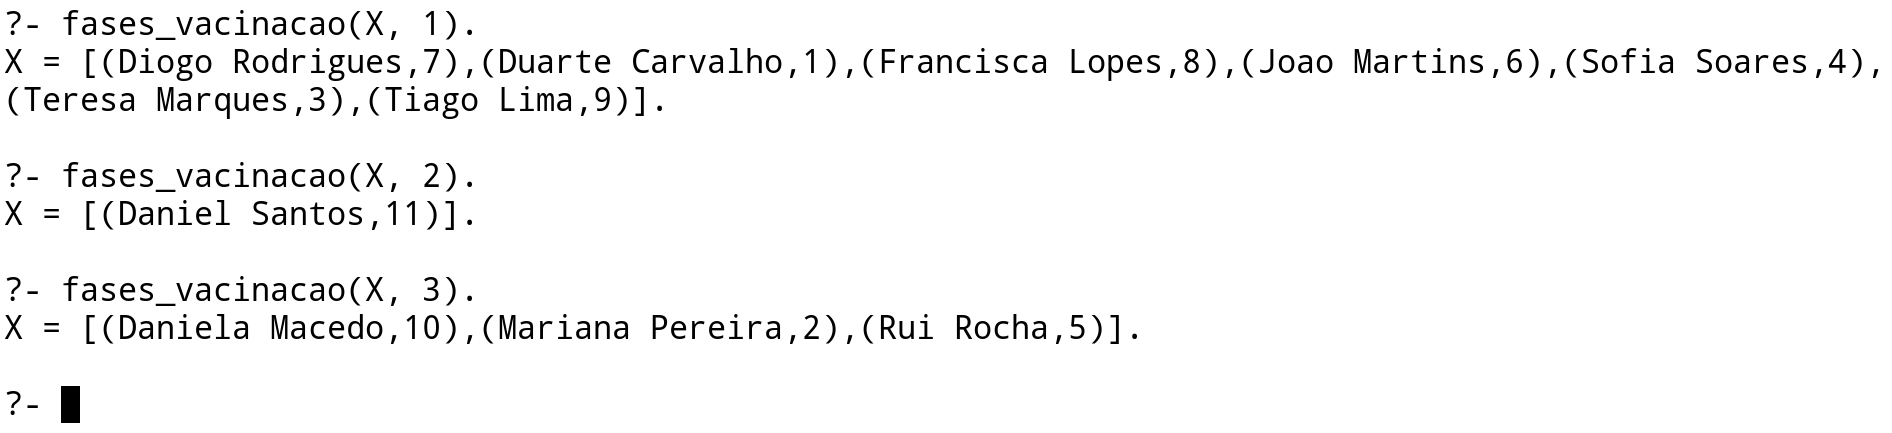
\includegraphics[width=\textwidth]{img/fases_vacinacao.png}
    \caption{Fases de vacinação}
\end{figure}

\subsubsection{Utentes Não Vacinados}

O seguinte predicado \texttt{nao\_vacinados} permite determinar o nome e respetivo ID dos utentes que ainda não foram
vacinadas com ambas as tomas da vacina.

\

\begin{lstlisting}[language=Prolog, caption={Extensão do predicado \texttt{nao\_vacinados}}]
% Extensao do predicado nao_vacinados: R -> {V, F}
nao_vacinados(R) :- 
    solucoes((NOME, ID), utente(ID, _, NOME, _, _, _, _, _, _, _), UT),
    solucoes((NOME, ID), (utente(ID, _, NOME, _, _, _, _, _, _, _),
                          vacinacao_Covid(_, ID, _, _, 2)), VAC),
    subtract(UT, VAC, L),
    sort(L, R).
\end{lstlisting}

\

\begin{figure}[H]
    \centering
    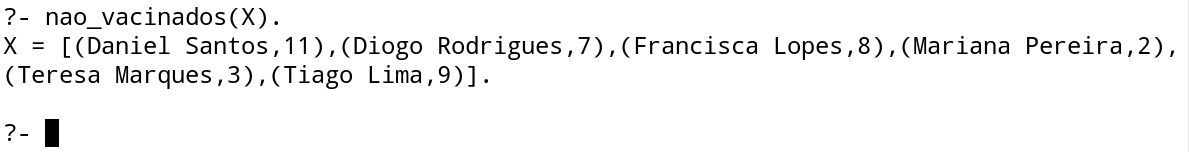
\includegraphics[width=.9\textwidth]{img/nao_vacinados.png}
    \caption{Utentes não vacinados}
\end{figure}

\subsubsection{Utentes Vacinados}

O predicado \texttt{vacinados} permite determinar o nome de respetivo ID dos utentes que levaram as duas tomas da vacina.

\

\begin{lstlisting}[language=Prolog, caption={Extensão do predicado \texttt{vacinados}}]
% Extensao do predicado vacinados: R -> {V, F}
vacinados(R) :- 
    solucoes((NOME, ID), (utente(ID, _, NOME, _, _, _, _, _, _, _),
                          vacinacao_Covid(_, ID, _, _, 2)), L),
    sort(L, R).
\end{lstlisting}

\

\begin{figure}[H]
    \centering
    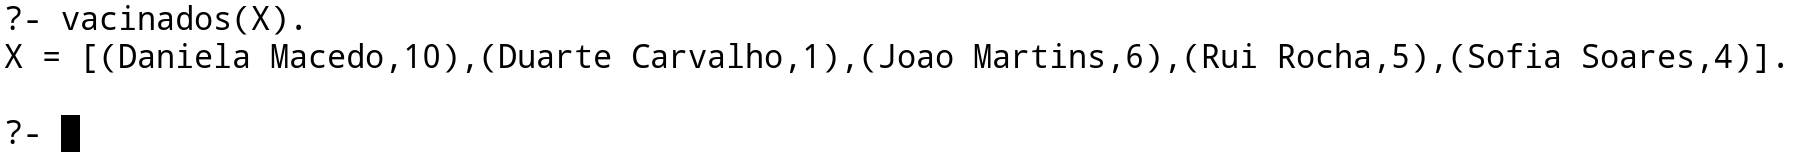
\includegraphics[width=\textwidth]{img/vacinados.png}
    \caption{Utentes vacinados}
\end{figure}

\subsubsection{Utentes Vacinados Indevidamente}

De forma a identificar quais os utentes que foram vacinados indevidamente, é, antes de mais, necessário identificar
em que fase de vacinação cada um dos utentes deve ser vacinado, assim como a fase atual de vacinação. Nesse sentido,
foram desenvolvidos o predicado \texttt{utente\_fase} e \texttt{fase\_atual}. Assim, considera-se que um utente foi
vacinado indevidamente se, apesar de já ter recebido um qualquer número de tomas da vacina, a fase em que este deve ser
vacinado é posterior à fase atual.

\

\begin{lstlisting}[language=Prolog, caption={Extensão do predicado \texttt{utente\_fase}}]
% Extensao do predicado utente_fase: ID, F -> {V, F}
utente_fase(ID, 1) :- 
    solucoes(ID, utente(ID, _, _, _, _, _, _, _, [_|_], _), L),
    comprimento(L, N),
    N == 1, !.

utente_fase(ID, 2) :-
    solucoes(ID, (utente(ID, _, _, DATA, _, _, _, _, _, _),
                  idade(DATA, I), I >= 65), L),
    comprimento(L, N),
    N == 1, !.

utente_fase(_, 3).
\end{lstlisting}

\

\begin{lstlisting}[language=Prolog, caption={Extensão do predicado \texttt{fase\_atual}}]
% Extensao do predicado fase_atual: F -> {V, F}
fase_atual(3) :- fases_vacinacao(F1, 1), fases_vacinacao(F2, 2),
                 concat(F1, F2, F),
                 vacinados(VAC),
                 subset(F, VAC).

fase_atual(2) :- fases_vacinacao(F1, 1),
                 vacinados(VAC),
                 subset(F1, VAC).

fase_atual(1).
\end{lstlisting}

\pagebreak

\begin{lstlisting}[language=Prolog, caption={Extensão do predicado \texttt{vacinados\_indevidamente}}]
% Extensao do predicado vacinados_indevidamente: R -> {V, F}
vacinados_indevidamente(R) :- 
    fase_atual(F),
    solucoes((NOME, ID), (utente(ID, _, NOME, _, _, _, _, _, _, _),
                          utente_fase(ID, FU), FU > F), S),
    sort(S, R).
\end{lstlisting}

\

\begin{figure}[H]
    \centering
    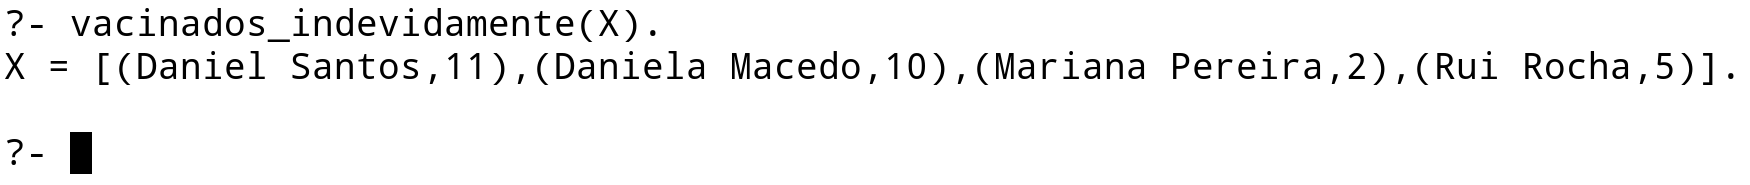
\includegraphics[width=\textwidth]{img/vacinados_indevidamente.png}
    \caption{Utentes vacinados indevidamente}
\end{figure}

\subsubsection{Utentes Não Vacinados Candidatos a Vacinação}

De forma a determinar os utentes não vacinados e que são candidatos à vacinação. Este predicado faz uso do predicado
\texttt{fase\_atual} definido anteriormente.

\

\begin{lstlisting}[language=Prolog, caption={Extensão do predicado \texttt{candidatos}}]
% Extensao do predicado candidatos: R -> {V, F}
candidatos(R) :- nao_vacinados(NV),
                 fase_atual(F),
                 solucoes((NOME, ID), 
                          (utente(ID, _, NOME, _, _, _, _, _, _, _),
                           utente_fase(ID, FU), FU == F), S),
                 intersection(NV, S, L),
                 sort(L, R).
\end{lstlisting}

\

\begin{figure}[H]
    \centering
    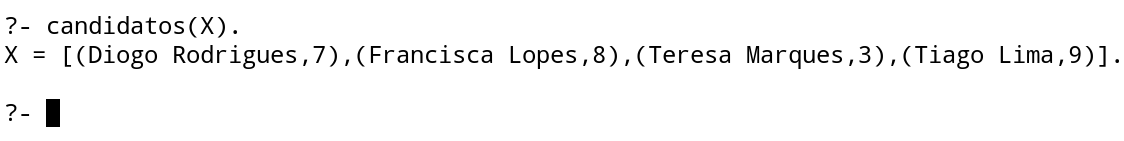
\includegraphics[width=\textwidth]{img/candidatos.png}
    \caption{Utentes candidatos a vacinação}
\end{figure}

\subsubsection{Utentes a Quem Falta a Segunda Toma da Vacina}

O seguinte predicado \texttt{falta\_segunda} permite determinar o nome e respetivo ID dos utentes a quem, apesar de
já terem sido vacinados com a primeira toma, ainda lhes falta ser administrada a segunda toma da vacina. 

\

\begin{lstlisting}[language=Prolog, caption={Extensão do predicado \texttt{falta\_segunda}}]
% Extensao do predicado falta_segunda: R -> {V, F}
falta_segunda(R) :- 
    solucoes((NOME, ID), (utente(ID, _, NOME, _, _, _, _, _, _, _),
                          vacinacao_Covid(_, ID, _, _, 1)), V1),
    solucoes((NOME, ID), (utente(ID, _, NOME, _, _, _, _, _, _, _),
                          vacinacao_Covid(_, ID, _, _, 2)), VAC),
    subtract(V1, VAC, L),
    sort(L, R).
\end{lstlisting}

\

\begin{figure}[H]
    \centering
    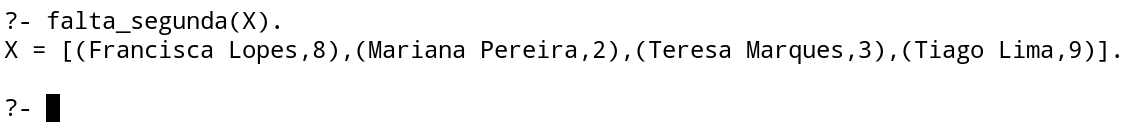
\includegraphics[width=.9\textwidth]{img/falta_segunda.png}
    \caption{Utentes a quem falta a segunda toma da vacina}
\end{figure}

\subsection{Predicados Extra}

Adicionalmente aos predicados essenciais a este exercício prático, foram desenvolvidos alguns predicados extra, pensando
na inclusão de novas funcionalidades de modo a pôr em prática todo o conhecimento adquirido. Estes predicados estão
maioritariamente relacionados com \textit{queries} de procura de informação na base de conhecimento.

De seguida enumeram-se e apresentam-se os predicados complementarmente desenvolvidos.

\subsubsection{Utentes Sem Doenças Crónicas}

O predicado \texttt{sem\_doencas\_cronicas} permite determinar o nome de respetivo ID dos utentes que não possuem
doenças crónicas.

\

\begin{lstlisting}[language=Prolog, caption={Extensão do predicado \texttt{sem\_doencas\_cronicas}}]
% Extensao do predicado sem_doencas_cronicas: R -> {V, F}
sem_doencas_cronicas(R) :- 
    solucoes((NOME, ID), utente(ID, _, NOME, _, _, _, _, _, [], _), UT),
    sort(UT, R).
\end{lstlisting}

\begin{figure}[H]
    \centering
    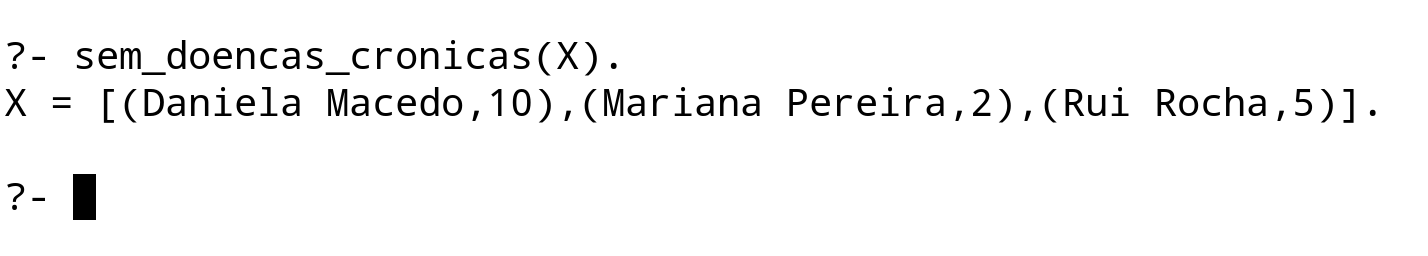
\includegraphics[width=.8\textwidth]{img/sem_doencas_cronicas.png}
    \caption{Utentes sem doenças crónicas}
\end{figure}

\subsubsection{Utentes}

O predicado \texttt{utentes} permite determinar o nome e respetivo ID de todos os utentes presentes na base de
conhecimento.

\

\begin{lstlisting}[language=Prolog, caption={Extensão do predicado \texttt{utentes}}]
% Extensao do predicado utentes: R -> {V, F}
utentes(R) :-  
    solucoes((NOME, ID), utente(ID, _, NOME, _, _, _, _, _, _, _), S),
    sort(S, R).
\end{lstlisting}

\

\begin{figure}[H]
    \centering
    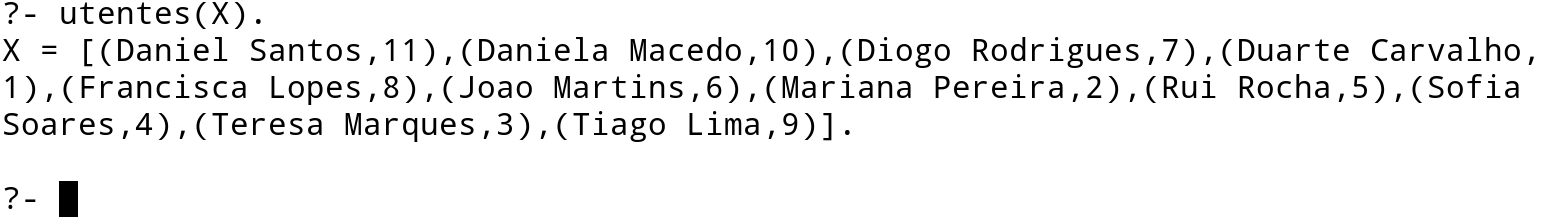
\includegraphics[width=\textwidth]{img/utentes.png}
    \caption{Utentes}
\end{figure}

\subsubsection{\textit{Staff}}

O predicado \texttt{staff} permite determinar o nome e respetivo ID de todos os elementos do \textit{staff} presentes
na base de conhecimento.

\

\begin{lstlisting}[language=Prolog, caption={Extensão do predicado \texttt{staff}}]
% Extensao do predicado staff: R -> {V, F}
staff(R) :- 
    solucoes((NOME, ID), staff(ID, _, NOME, _), S),
    sort(S, R).
\end{lstlisting}

\

\begin{figure}[H]
    \centering
    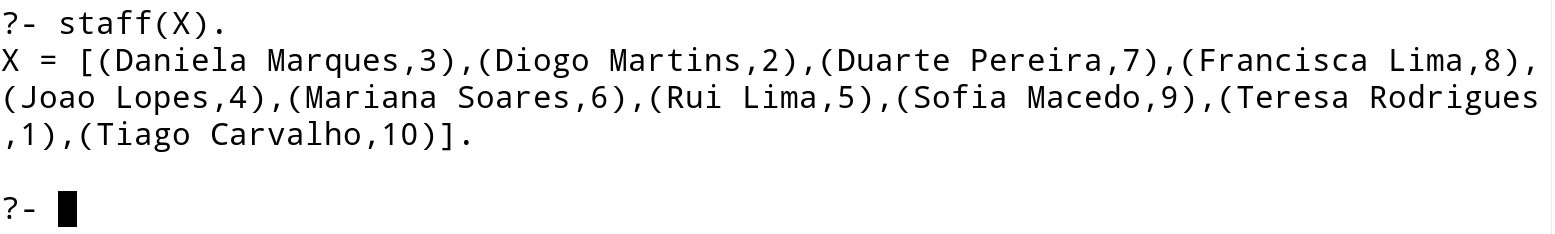
\includegraphics[width=\textwidth]{img/staff.png}
    \caption{\textit{Staff}}
\end{figure}

\subsubsection{Centros de Saúde}

O predicado \texttt{centros\_saude} permite determinar o nome de todos os centros de saúde presentes na base
de conhecimento.

\

\begin{lstlisting}[language=Prolog, caption={Extensão do predicado \texttt{centros\_saude}}]
% Extensao do predicado centros_saude: R -> {V, F}
centros_saude(R) :- 
    solucoes(NOME, centro_saude(_, NOME, _, _, _), S),
    sort(S, R).
\end{lstlisting}

\

\begin{figure}[H]
    \centering
    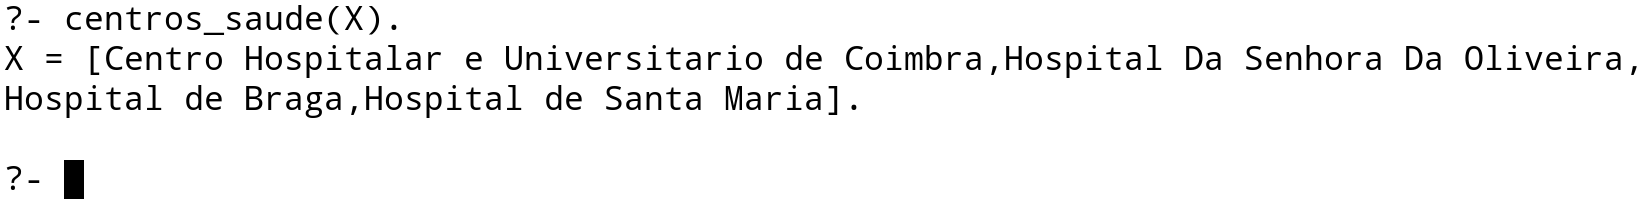
\includegraphics[width=\textwidth]{img/centros_saude.png}
    \caption{Centros de saúde}
\end{figure}

\subsubsection{Médicos}

O predicado \texttt{medicos} permite determinar o nome e respetivo ID de todos os utentes presentes na base
de conhecimento.

\

\begin{lstlisting}[language=Prolog, caption={Extensão do predicado \texttt{medicos}}]
% Extensao do predicado medicos: R -> {V, F}
medicos(R) :- 
    solucoes((NOME, ID), medico(ID, _, NOME, _, _), S),
    sort(S, R).
\end{lstlisting}

\

\begin{figure}[H]
    \centering
    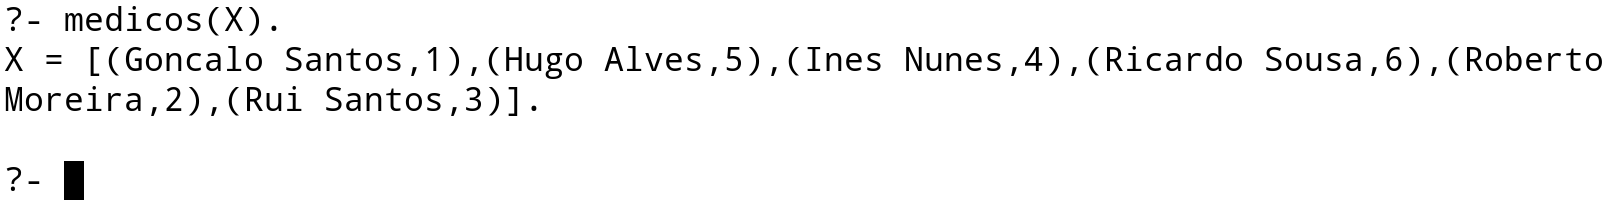
\includegraphics[width=\textwidth]{img/medicos.png}
    \caption{Médicos}
\end{figure}

\subsubsection{Médicos de uma Especialidade}

O predicado \texttt{medicos\_especialidade} permite determinar os médicos que exercem uma determinada especialidade.

\

\begin{lstlisting}[language=Prolog, caption={Extensão do predicado \texttt{medicos\_especialidade}}]
% Extensao do predicado medicos_especialidade: ESP, R -> {V, F}
medicos_especialidade(ESP, R) :- 
    solucoes((NOME, ID), medico(ID, _, NOME, _, ESP), L),
    sort(L, R).
\end{lstlisting}

\

\begin{figure}[H]
    \centering
    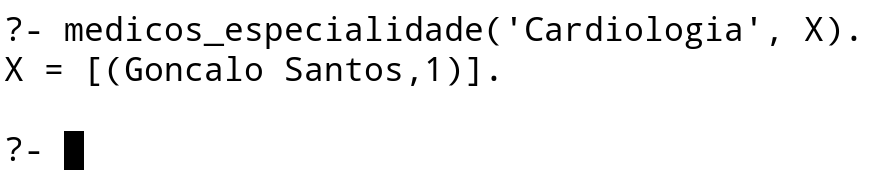
\includegraphics[width=.55\textwidth]{img/cardiologia.png}
    \caption{Médicos cardiologistas}
\end{figure}

\subsubsection{Especialidades Médicas}

O predicado \texttt{especialidades} permite determinar as especialidades médicas disponíveis num determinado
centro de saúde.

\

\begin{lstlisting}[language=Prolog, caption={Extensão do predicado \texttt{especialidades}}]
% Extensao do predicado especialidades: IDC, R -> {V, F}
especialidades(IDC, R) :- 
    solucoes(ESP, medico(_, IDC, _, _, ESP), L),
    list_to_set(L, S),
    sort(S, R).
\end{lstlisting}

\

\begin{figure}[H]
    \centering
    
\includegraphics[width=.45\textwidth]{img/especialidades.png}
    \caption{Especialidades médicas disponíveis no centro de saúde \#3}
\end{figure}

\subsubsection{Utentes de um Centro de Saúde}

Fazendo uso do predicado \texttt{utentes\_centro}, é possível determinar o nome e respetivo ID dos utentes que
frequentam um determinado centro de saúde.

\

\begin{lstlisting}[language=Prolog, caption={Extensão do predicado \texttt{utentes\_centro}}]
% Extensao do predicado utentes_centro: IDC, R -> {V, F}
utentes_centro(IDC, R) :- 
    solucoes((NOME, ID), utente(ID, _, NOME, _, _, _, _, _, _, IDC), L),
    sort(L, R).
\end{lstlisting}

\

\begin{figure}[H]
    \centering
    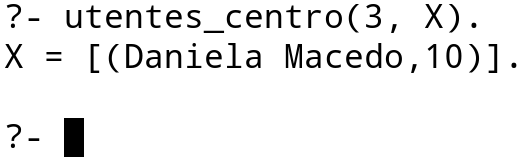
\includegraphics[width=.35\textwidth]{img/utentes_centro.png}
    \caption{Utentes que frequentam o centro de saúde \#3}
\end{figure}

\subsubsection{\textit{Staff} de um Centro de Saúde}

Fazendo uso do predicado \texttt{staff\_centro}, é possível determinar o nome e respetivo ID dos elementos do
\textit{staff} que exercem funções num determinado centro de saúde.

\

\begin{lstlisting}[language=Prolog, caption={Extensão do predicado \texttt{staff\_centro}}]
% Extensao do predicado staff_centro: IDC, R -> {V, F}
staff_centro(IDC, R) :- 
    solucoes((NOME, ID), staff(ID, IDC, NOME, _), L),
    sort(L, R).
\end{lstlisting}

\

\begin{figure}[H]
    \centering
    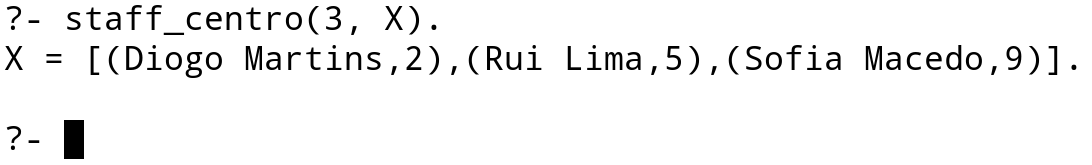
\includegraphics[width=.7\textwidth]{img/staff_centro.png}
    \caption{\textit{Staff} do centro de saúde \#3}
\end{figure}

\subsubsection{Médicos de um Centro de Saúde}

Fazendo uso do predicado \texttt{medicos\_centro}, é possível determinar o nome e respetivo ID dos médicos que exercem
funções num determinado centro de saúde.

\begin{lstlisting}[language=Prolog, caption={Extensão do predicado \texttt{medicos\_centro}}]
% Extensao do predicado medicos_centro: IDC, R -> {V, F}
medicos_centro(IDC, R) :- 
    solucoes((NOME, ID), medico(ID, IDC, NOME, _, _), L),
    sort(L, R).
\end{lstlisting}

\

\begin{figure}[H]
    \centering
    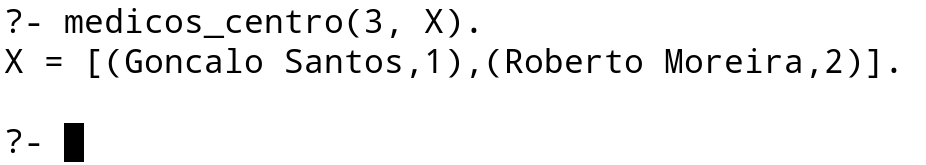
\includegraphics[width=.65\textwidth]{img/medicos_centro.png}
    \caption{Médicos que exercem funções no centro de saúde \#3}
\end{figure}

\subsubsection{Guardar e carregar a base de conhecimento através  da utilização de um ficheiro de texto}

Aquando da realização de diversos testes, constatou-se que as alterações aplicadas à base de conhecimento (inserção e
remoção de factos) apenas se mantêm em tempo de execução, sendo que no final da execução do interpretador, todas estas
alterações são apagadas.

Assim, uma vez que é conveniente guardar de algum modo todos os factos referentes aos  diversos predicados para, assim,
permitir a evolução da base de conhecimento sem que seja perdida nenhuma informação, foi desenvolvido o predicado \texttt{save},
que guarda estado atual da base de conhecimento no ficheiro \texttt{knowledge.pl}, sendo este novamente carregado quando
o programa é executado.

\pagebreak

\subsection{Sistema de Inferência}

Aquando da resolução do trabalho prático, tornou-se essencial construir um sistema de inferência capaz de implementar
os mecanismos de raciocínio inerentes a este sistema, descrito em seguida.

De forma a implementar este sistema de inferência, foi necessário construir o meta-predicado \texttt{nao}, que devolve
o valor de verdade contrário ao do termo passado como parâmetro através da negação fraca.


\

\begin{lstlisting}[language=Prolog, caption={Sistema de Inferência}]
% Extensao do meta-predicado nao: Questao -> {V,F}
nao(Questao) :- Questao, !, fail.
nao(_).

% Extensao do meta-predicado si: Questao, Resposta -> {V,F}
si(Questao, verdadeiro) :- Questao.
si(Questao, falso) :- -Questao.
\end{lstlisting}

A título de exemplo, considere-se o seguinte predicados que permite, dado o ID de um utente, determinar se este foi
ou não vacinado.

\

\begin{lstlisting}[language=Prolog, caption={Predicados que permitem determinar se um utente foi vacinado}]
% Extensao do predicado vacinado: ID -> {V, F}
vacinado(ID) :- 
    solucoes(ID, (utente(ID, _, _, _, _, _, _, _, _, _),
                  vacinacao_Covid(_, ID, _, _, 2)), S),
    comprimento(S, N),
    N == 1.

-vacinado(ID) :- nao(vacinado(ID)).
\end{lstlisting}

\ 

Assim, utilizando o sistema de inferência desenvolvido, é possível verficiar o valor de verdade associado a esta questão.

\begin{figure}[H]
    \centering
    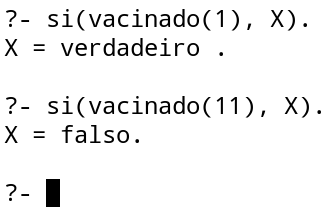
\includegraphics[width=.27\textwidth]{img/si.png}
    \caption{Sistema de Inferência}
\end{figure}

\pagebreak

\section{Conclusão e Trabalho Futuro}

De uma forma geral, consideramos que o objetivo do trabalho prático foi concluído. Foram implementadas todas as funcionalidades
solicitadas de forma a permitir uma representação do conhecimento, com vários exemplos e demonstrações de cada um deles.
Os invariantes necessários foram pensados ao pormenor para uma correta manipulação da base de conhecimento, tanto para o
caso da inserção como para a remoção de conhecimento. Efetivamente, para além de ser dada resposta a todas as interrogações,
foi também possível elaborar alguns predicados extra que consideramos ser relevantes.

Como trabalho futuro, poderiam ser implementados predicados de modo a permitir a atualização de certas informações das
entidades envolvidas que, ao longo do tempo, podem vir a tornar-se desatualizadas.

\pagebreak

\renewcommand\bibname{Referências}
\begin{thebibliography}{2}

\section*{Referências Bibliográficas}

\bibitem{analide} 
ANALIDE, Cesar, NOVAIS, Paulo, Neves, José\\
"Sugestões para a Redacção de Relatórios Técnicos"\\
Relatório Técnico, Departamento de Informática, Universidade do Minho, Portugal, 2011

\end{thebibliography}

\pagebreak

\appendix

\pagebreak

\section{Predicados Auxiliares}

\subsection*{Meta-predicado \texttt{comprimento}}

O meta-predicado \texttt{comprimento} é utilizado sempre que se pretende obter informação relativamente ao tamanho de
uma dada lista. 

\

\begin{lstlisting}[language=Prolog, caption={Extensão do meta-predicado \texttt{comprimento}}]
% Extensao do predicado comprimento: S, N -> {V, F}
comprimento(S, N) :- length(S, N).
\end{lstlisting}

\subsection*{Meta-predicado \texttt{solucoes}}

Utiliza-se este predicado quando se pretende obter a listagem de todas as soluções possíveis \texttt{Z}, para uma dada questão
\texttt{Y}, cujo formato da lista é especificado por \texttt{X}. Faz-se uso do predicado disponibilizado pelo \texttt{PROLOG},
\texttt{findall}, uma vez que este não falha na eventualidade de não existir resposta a esta questão, ao contrário do
que aconteceria com o predicado \texttt{bagof}.

\

\begin{lstlisting}[language=Prolog, caption={Extensão do meta-predicado \texttt{solucoes}}]
% Extensao do meta-predicado solucoes: X, Y, Z -> {V, F}
solucoes(X, Y, Z) :- findall(X, Y, Z).
\end{lstlisting}

\subsection*{Meta-predicado \texttt{teste}}

Utiliza-se este predicado quando se pretende verificar se todas as questões
existentes numa lista são verdadeiras, que é conseguido através da implementação de recorrência.

\

\begin{lstlisting}[language=Prolog, caption={Extensão do meta-predicado \texttt{teste}}]
% Extensao do meta-predicado teste: L -> {V, F}
teste([]).
teste([H|T]) :- H, teste(T).
\end{lstlisting}

\pagebreak

\subsection*{Idade de um Utente}

Para determinar em que fase de vacinação um determinado utente deve ser incluído, é necessário determinar a sua idade.
Nesse sentido, e recorrendo a um conjunto de predicados auxiliares, foi desenvolvido o seguinte predicado \texttt{idade}.

\

\begin{lstlisting}[language=Prolog, caption={Predicados auxiliares que permitem determinar a idade de um utente}]
% Extensao do predicado year: date(Y, M , D), R -> {V, F}
year(date(Y, _, _), Y).

% Extensao do predicado month: date(Y, M , D), R -> {V, F}
month(date(_, M, _), M).

% Extensao do predicado day: date(Y, M , D), R -> {V, F}
day(date(_, _, D), D).

% Extensao do predicado years_between_dates: D1, D2, R -> {V, F}
years_between_dates(D1, D2, R):- year(D1, Y1), year(D2, Y2),
                                 month(D1, M1), month(D2, M2),
                                 M2 > M1, R is Y2 - Y1.
                                 
years_between_dates(D1, D2, R):- year(D1, Y1), year(D2,Y2),
                                 month(D1, M1), month(D2, M2),
                                 day(D1, DAY1), day(D2, DAY2),
                                 M2 == M1, DAY2 >= DAY1, R is Y2 - Y1.
                                 
years_between_dates(D1, D2, R):- year(D1, Y1), year(D2, Y2),
                                 R is Y2 - Y1-1.

% Extensao do predicado format_date:
%    date(Y, M, D, H, Mn, S, Off, TZ, DST), date(Y, M, D) -> {V, F}
format_date(date(Y, M, D, _, _, _, _, _, _), date(Y, M, D)).

% Extensao do predicado current_date: Date -> {V, F}
current_date(Date) :- get_time(Stamp),
                      stamp_date_time(Stamp, DateTime, local),
                      format_date(DateTime, Date).

% Extensao do predicado idade: Data_Nasc, Idade -> {V, F}
idade(Data_Nasc, Idade) :- 
    current_date(Date), years_between_dates(Data_Nasc, Date, Idade).
\end{lstlisting}

\pagebreak

\section{Povoamento Inicial da Base de Conhecimento}

\begin{lstlisting}[language=Prolog, caption={Base de conhecimento de \texttt{utente}}]
% Extensao do predicado utente: #Idutente, No Seguranca_Social, Nome,
                                Data_Nasc, Email, Telefone, Morada,
                                Profissao, [Doencas_Cronicas],
                                #CentroSaude -> {V, F}

utente(1, 14492, 'Duarte Carvalho', date(1998,4,21),
       'duartecarvalho@gmail.com', 91761416, 'Lisboa', 'Estudante',
      ['Asma'], 4).
utente(2, 95110, 'Mariana Pereira', date(1988,11,12),
       'marianapereira@gmail.com', 915992520, 'Porto', 'Atleta', [], 4).      
utente(3, 79297, 'Teresa Marques', date(1987,8,30),
       'teresamarques@gmail.com', 913844675, 'Viseu', 'Engenheira',
       ['Hipertensao'], 4).      
utente(4, 71723, 'Sofia Soares', date(1979,6,8), 'sofiasoares@gmail.com',
       919555582, 'Porto', 'Advogada', ['Diabetes'], 2).      
utente(5, 40203, 'Rui Rocha', date(1987,12,24), 'ruirocha@gmail.com',
       919219565, 'Braga', 'Atleta', [], 1).      
utente(6, 77645, 'Joao Martins', date(1998,11,12), 'joaomartins@gmail.com
       ', 917630282, 'Coimbra', 'Estudante', ['Asma'], 2).      
utente(7, 67275, 'Diogo Rodrigues', date(1995,1,25),
       'diogorodrigues@gmail.com', 916543686, 'Lisboa', 'Engenheiro',
       ['Diabetes','Cancro'], 2).      
utente(8, 76991, 'Francisca Lopes', date(1986,9,15),
       'franciscalopes@gmail.com', 913672965, 'Braga', 'Enfermeira',
       ['Asma'], 2).
utente(9, 82539, 'Tiago Lima', date(1978,12,12), 'tiagolima@gmail.com',
       91683448, 'Lisboa', 'Medico', ['Hipertensao'], 5).      
utente(10, 16086, 'Daniela Macedo', date(1977,10,25),
       'danielamacedo@gmail.com', 911216397, 'Coimbra', 'Medico', [], 3).
utente(11, 56418, 'Daniel Santos', date(1955, 2, 23),
       'danielsantos@gmail.com', 915632478, 'Faro', 'Advogado', [], 4).
\end{lstlisting}

\

\begin{lstlisting}[language=Prolog, caption={Base de conhecimento de \texttt{centro\_saude}}]
% Extensao do predicado centro_saude: #Idcentro, Nome, Morada, Telefone,
                                      Email -> {V, F}
                                      
centro_saude(1, 'Hospital de Braga', 'Braga', 253027000,
             'hospitaldebraga@gmail.com').
centro_saude(2, 'Hospital Da Senhora Da Oliveira', 'Guimaraes',
             253540330, 'hospitaldasenhoradaoliveira@gmail.com').
centro_saude(3, 'Centro Hospitalar e Universitario de Coimbra',
             'Coimbra', 239400400,
             'centrohospitalareuniversitariodecoimbra@gmail.com').
centro_saude(4, 'Hospital de Santa Maria', 'Lisboa', 217805000,
             'hospitaldesantamaria@gmail.com').
\end{lstlisting}

\pagebreak

\begin{lstlisting}[language=Prolog, caption={Base de conhecimento de \texttt{staff}}]
% Extensao do predicado staff: #Idstaff, #Idcentro, Nome, email -> {V, F}

staff(1, 4, 'Teresa Rodrigues', 'teresarodrigues@gmail.com').
staff(2, 3, 'Diogo Martins', 'diogomartins@gmail.com').
staff(3, 2, 'Daniela Marques', 'danielamarques@gmail.com').
staff(4, 2, 'Joao Lopes', 'joaolopes@gmail.com').
staff(5, 3, 'Rui Lima', 'ruilima@gmail.com').
staff(6, 4, 'Mariana Soares', 'marianasoares@gmail.com').
staff(7, 1, 'Duarte Pereira', 'duartepereira@gmail.com').
staff(8, 4, 'Francisca Lima', 'franciscalima@gmail.com').
staff(9, 3, 'Sofia Macedo', 'sofiamacedo@gmail.com').
staff(10, 1, 'Tiago Carvalho', 'tiagocarvalho@gmail.com').
\end{lstlisting}

\vspace{3.5cm}

\begin{lstlisting}[language=Prolog, caption={Base de conhecimento de \texttt{vacinacao\_Covid}}]
% Extensao do predicado vacinacao_Covid: #Idstaff, #Idutente, Data,
                                         Vacina, Toma -> {V, F}
                                         
vacinacao_Covid(7, 1, date(2021,4,23), 'Pfizer', 1).
vacinacao_Covid(5, 1, date(2021,8,24), 'Pfizer', 2).
vacinacao_Covid(7, 2, date(2020,2,1), 'Astrazeneca', 1).
vacinacao_Covid(10, 3, date(2020,10,13), 'Pfizer', 1).
vacinacao_Covid(9, 4, date(2020,11,11), 'Pfizer', 1).
vacinacao_Covid(6, 4, date(2020,12,19), 'Pfizer', 2).
vacinacao_Covid(1, 5, date(2020,3,21), 'Astrazeneca', 1).
vacinacao_Covid(5, 5, date(2020,7,30), 'Astrazeneca', 2).
vacinacao_Covid(8, 6, date(2020,5,3), 'Pfizer', 1).
vacinacao_Covid(7, 6, date(2020,10,20), 'Pfizer', 2).
vacinacao_Covid(7, 8, date(2021,7,17), 'Pfizer', 1).
vacinacao_Covid(9, 9, date(2020,2,21), 'Astrazeneca', 1).
vacinacao_Covid(3, 10, date(2020,9,29), 'Pfizer', 1).
vacinacao_Covid(1, 10, date(2020,12,13), 'Pfizer', 2).
\end{lstlisting}

\pagebreak

\begin{lstlisting}[language=Prolog, caption={Base de conhecimento de \texttt{medico}}]
% Extensao do predicado medico: #Idmedico, #Idcentro, Nome, Email,
                                Especialidade -> {V, F}

medico(1, 3, 'Goncalo Santos', 'goncalosantos@gmail.com', 'Cardiologia').
medico(2, 3, 'Roberto Moreira', 'robertomoreira@gmail.com',
       'Anestesiologia').
medico(3, 4, 'Rui Santos', 'ruisantos@gmail.com', 'Clinica Geral').
medico(4, 2, 'Ines Nunes', 'inesnunes@gmail.com', 'Dermatologia').
medico(5, 1, 'Hugo Alves', 'hugoalves@gmail.com', 'Gastrenterologia').
medico(6, 1, 'Ricardo Sousa', 'ricardosousa@gmail.com',
       'Medicina Dentaria').
\end{lstlisting}

\vspace{1.5cm}

\begin{lstlisting}[language=Prolog, caption={Base de conhecimento de \texttt{consulta}}]
% Extensao do predicado consulta: #Idmedico, #Idutente, #Idcentro, 
                                  Data -> {V, F}

consulta(3, 1, 4, date(2020,10,15)).
consulta(6, 5, 1, date(2021,3,2)).
consulta(4, 8, 2, date(2020,12,20)).
consulta(3, 2, 4, date(2020,8,14)).
\end{lstlisting}

\vspace{1.5cm}

\begin{lstlisting}[language=Prolog, caption={Base de conhecimento de \texttt{tratamento}}]
% Extensao do predicado tratamento: #IdStaff, #Idutente, #Idcentro, Data,
                                    Descricao -> {V, F}

tratamento(4, 4, 2, date(2021,3,14), 'Radiografia Perna').
tratamento(6, 1, 4, date(2021,2,1), 'Eletrocardiograma').
tratamento(7, 5, 1, date(2020,5,14), 'Exame Pulmonar').
tratamento(3, 8, 2, date(2021,3,1), 'Analises Clinicas').
\end{lstlisting}

\end{document}
